\section{Specyfikacja wymagań funkcjonalnych~i~niefunkcjonalnych}
\label{sec:wymagania}
%%%%%%%%%%%%%%%%%%%%%%%%%%%%%%%%%%%%%%%%%%%%%%%%%%%%%%%%%%%%%%%%%%%
\subsection{Wymagania funkcjonalne}
\begin{table}[H]
    \begin{tabular}{|l|l|} 
    \hline
    Id: F1              & \begin{tabular}[c]{@{}l@{}}Nazwa: Identyfikacja zaszyfrowanego pliku metodą pola między \\wykresami entropii\end{tabular}                                               \\ 
    \hline
    Warunek rozpoczęcia & Skan został zainicjowany na dowolny sposób                                                                                                                              \\ 
    \hline
    Warunki zakończenia & \begin{tabular}[c]{@{}l@{}}Sukces: wynik został zwrócony\\ Porażka: wynik nie został zwrócony\end{tabular}  \\
    \hline
    \end{tabular}
\end{table}

\begin{table}[H]
    \begin{tabular}{|l|l|} 
    \hline
    Id: F2              & Nazwa: Identyfikacja ransomware poprzez podobieństwo cos                                                           \\ 
    \hline
    Warunek rozpoczęcia & \begin{tabular}[c]{@{}l@{}}Skan został zainicjowany~i~sprawdzone zostało to czy plik jest \\typu ELF\end{tabular}  \\ 
    \hline
    Warunki zakończenia & \begin{tabular}[c]{@{}l@{}}Sukces: wynik został zwrócony\\ Porażka: wynik nie został zwrócony\end{tabular}         \\
    \hline
    \end{tabular}
\end{table}

\begin{table}[H]
    \begin{tabular}{|l|l|}
    \hline
    Id: F3              & Nazwa: Analiza ruchu metodą ilości dokonanych operacji                                                                                                                                                                                           \\ \hline
    Warunek rozpoczęcia & Zainicjowana została rutynowa kontrola                                                                                                                                                                                                           \\ \hline
    Warunki zakończenia & \begin{tabular}[c]{@{}l@{}}Sukces: czas wykonania operacji mieści się~w~przedziale\\czasowym zdefiniowanym~w~konfiguracji~i~przekracza \\ ilość operacji zdefiniowaną~w~konfiguracji.\\ Porażka: niemożliwe było odczytanie danych z bazy.\end{tabular} \\ \hline
    \end{tabular}
\end{table}


\begin{table}[H]
    \begin{tabular}{|l|l|}
    \hline
    Id: F4              & Nazwa: Analiza ruchu metodą ilości zmienionych nazw plików                                                                                                                                                                                           \\ \hline
    Warunek rozpoczęcia & Zainicjowana została rutynowa kontrola                                                                                                                                                                                                           \\ \hline
    Warunki zakończenia & \begin{tabular}[c]{@{}l@{}}Sukces: czas wykonania operacji mieści się~w~przedziale\\czasowym zdefiniowanym~w~konfiguracji~i~przekracza \\ ilość operacji zdefiniowaną~w~konfiguracji.\\ Porażka: niemożliwe było odczytanie danych z bazy.\end{tabular} \\ \hline
\end{tabular}
\end{table}

\begin{table}[H]
    \begin{tabular}{|l|l|} 
    \hline
    Id: F5              & \begin{tabular}[c]{@{}l@{}}Nazwa: Analiza ruchu metodą powstania plików zawierających\\słowa kluczowe (ransom notes)\end{tabular}                                                                                                                 \\ 
    \hline
    Warunek rozpoczęcia & Zainicjowana została rutynowa kontrola                                                                                                                                                                                                            \\ 
    \hline
    Warunki zakończenia & \begin{tabular}[c]{@{}l@{}}Sukces: wykryty został plik~i~zidentyfikowany jako ransom note. \\ Porażka: niemożliwe było odczytanie danych z bazy lub plik \\ nie został wykryty mimo obecności danych o tym świadczących.\end{tabular}  \\
    \hline
    \end{tabular}
    \end{table}

\begin{table}[H]
        \begin{tabular}{|l|l|}
        \hline
        Id: F6              & Nazwa: Analiza ruchu konfigurowalnym rutynowym skanem                                                                                                                                                                                           \\ \hline
        Warunek rozpoczęcia & Zainicjowana została rutynowa kontrola                                                                                                                                                                                                           \\ \hline
        Warunki zakończenia & \begin{tabular}[c]{@{}l@{}}Sukces: skan został wykonany o czasie zdefiniowanym~w~konfiguracji. \\ Porażka: skan się nie odbył~w~sprecyzowanym czasie lub interwale.\end{tabular} \\ \hline
\end{tabular}
\end{table}

\begin{table}[H]
    \begin{tabular}{|l|l|}
    \hline
    Id: F7              & Nazwa:  Wysyłanie powiadomień na serwer \texttt{syslog}                                                                                \\ \hline
    Warunek rozpoczęcia & Zakończony został skan                                                                                                                                  \\ \hline
    Warunki zakończenia & \begin{tabular}[c]{@{}l@{}}Sukces: raport o skanie został wysłany na serwer syslog.\\ Porażka: raport nie został wysłany na serwer syslog.\end{tabular} \\ \hline
    \end{tabular}
\end{table}
%%%%%%%%%%%%%%%%%%%%%%%%%%%%%%%%%%%%%%%%%%%%%%%%%%%%%%%%%%%%%%%%%%%
\subsection{Wymagania jakościowe}
\begin{table}[H]
    \begin{tabular}{|ll|}
    \hline
    \multicolumn{1}{|l|}{ID: J1}                                                          & \begin{tabular}[c]{@{}l@{}}Nazwa:  Komponent kolekcjonowania operacji powinien być wspierany przez \\ najważniejsze dystrybucje\end{tabular}                                                        \\ \hline
    \multicolumn{2}{|l|}{Rodzaj: przenośność}                                                                                                                                                                                                                                                   \\ \hline
    \multicolumn{2}{|l|}{\begin{tabular}[c]{@{}l@{}}Opis: Aby aplikacja mogła być użyteczna dla administratorów, element odpowiadający \\ za zbieranie informacji o systemie plików musi być możliwy do użycia na popularnych\\ dystrybucjach serwerowych systemu Linux.\end{tabular}}          \\ \hline
    \multicolumn{2}{|l|}{\begin{tabular}[c]{@{}l@{}}Sposób pomiaru: Technologia wykorzystywana do zbierania informacji musi być dostępna \\ na Ubuntu 22.04.1 LTS Server, RHEL 8.8, RHEL 7.9, Open SUSE Leap 15.5 oraz SUSE \\ Linux Enterprise Server 12.\end{tabular}}                        \\ \hline
    \multicolumn{2}{|l|}{Możliwy wynik pomiaru: Funkcjonalność na danym systemie jest albo nie jest wspierana.}                                                                                                                                                                                 \\ \hline
    \multicolumn{2}{|l|}{\begin{tabular}[c]{@{}l@{}}Oczekiwanie wartości: Możliwe są tylko dwie wartości. Albo wszystkie dystrybucje wspierają \\ funkcjonalność, albo nie. Gdy chociaż jedna dystrybucja nie wspiera funkcjonalności, wymóg \\ jakościowy nie został spełniony.\end{tabular}} \\ \hline
    \end{tabular}
\end{table}
 
\begin{table}[H]
    \begin{tabular}{|ll|}
    \hline
    \multicolumn{1}{|l|}{ID: J2}                                                                                                                 & Nazwa:  Instalacja musi być bezinwazyjna                                                                                                               \\ \hline
    \multicolumn{2}{|l|}{Rodzaj: przydatność funkcjonalna}                                                                                                                                                                                                                                                \\ \hline
    \multicolumn{2}{|l|}{\begin{tabular}[c]{@{}l@{}}Opis: Instalacja nie może wymagać instalacji dodatkowych pakietów, zmiany \\ integralnych ustawienień sytemowych ani ponownego uruchamiania systemu.\end{tabular}}                                                                                  \\ \hline
    \multicolumn{2}{|l|}{\begin{tabular}[c]{@{}l@{}}Sposób pomiaru: Należy przejść przez proces instalacji~i~sprawdzić, czy \\ będzie on wymagał ponownego uruchomienia systemu lub przeładowania \\ modułów jądra systemu.\end{tabular}}                                                         \\ \hline
    \multicolumn{2}{|l|}{\begin{tabular}[c]{@{}l@{}}Możliwy wynik pomiaru: Operacja uruchomienia ponownego~i~przeładowania\\ modułów jądra systemu jest albo nie jest potrzebna przy instalacji.\end{tabular}}                                                                                            \\ \hline
    \multicolumn{2}{|l|}{\begin{tabular}[c]{@{}l@{}}Oczekiwanie wartości: Możliwe są tylko dwie wartości. Albo proces \\ wymaga naruszenia działania systemu albo nie. Jeśli wcześniej wymienione \\ działania są potrzebne~w~procesie instalacji, wymóg jakościowy nie został\\ spełniony.\end{tabular}} \\ \hline
    \end{tabular}
\end{table}

\begin{table}[H]
    \begin{tabular}{|ll|}
    \hline
    \multicolumn{1}{|l|}{ID: J3}                                                                                                                                    & Nazwa: Niskie zużycie zasobów                                                                                                                                   \\ \hline
    \multicolumn{2}{|l|}{Rodzaj: efektywność wydajnościowa}                                                                                                                                                                                                                                                                           \\ \hline
    \multicolumn{2}{|l|}{\begin{tabular}[c]{@{}l@{}}Opis: Aplikacja nie może nadwyrężać zasobów systemu~w~sposób, który\\ znacząco zmniejszałby jego możliwości obliczeniowe.\end{tabular}}                                                                                                                                           \\ \hline
    \multicolumn{2}{|l|}{\begin{tabular}[c]{@{}l@{}}Sposób pomiaru: Aplikacja powinna nie zużywać więcej niż 15\% CPU\\ dla 180 tysięcy operacji na systemie plików. Należy doprowadzić system\\ do wykonania 180 tysięcy operacji~z~pomiarem zużycia CPU.\\ Następnie powtórzyć go 10 razy~i~wyciągnąć medianę.\end{tabular}} \\ \hline
    \multicolumn{2}{|l|}{\begin{tabular}[c]{@{}l@{}}Możliwy wynik pomiaru: Zużycie mierzymy od rozpoczęcia pierwszej \\ do zakończenia ostatniej operacji. Liczy się najwyższe zużycie z całego \\ przedziału czasowego.\end{tabular}}                                                                                                \\ \hline
    \multicolumn{2}{|l|}{\begin{tabular}[c]{@{}l@{}}Oczekiwanie wartości: Mediana może przekroczyć zużycie maksymalne\\ najwyżej o 1.5 \%.~W~innym wypadku wymóg jakościowy nie został spełniony.\end{tabular}}                                                                                                                             \\ \hline
    \end{tabular}
\end{table}
%%%%%%%%%%%%%%%%%%%%%%%%%%%%%%%%%%%%%%%%%%%%%%%%%%%%%%%%%%%%%%%%%%%
\newpage
\section{Sposób zbierania~i~przetwarzania statystyk systemu plików}
Mając na uwadze wymagania z sekcji \hyperref[sec:wymagania]{Specyfikacja wymagań funkcjonalnych~i~niefunkcjonalnych}, jako silnik obserwowania operacji na systemie plików wybrałem, przedstawiony~w~\hyperref[sec:auditd]{podsekcji drugiej podrozdziału Monitorowanie zmian na systemie plików} - Linux Auditing Framework.
\begin{figure}[H]
    \centering
    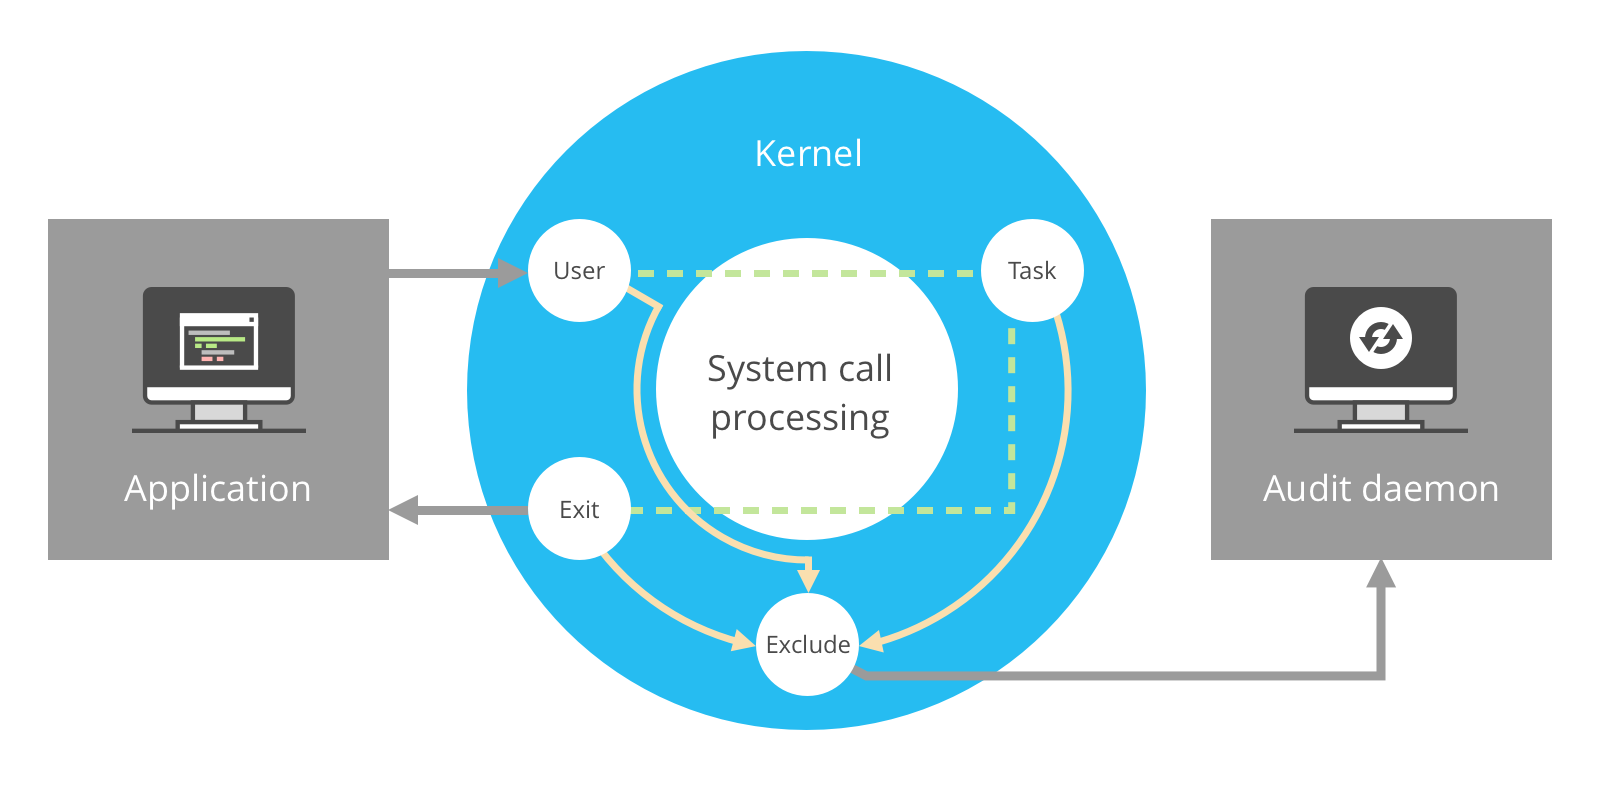
\includegraphics[width=0.9\linewidth]{rysunki/auditing.png}
    \caption{Diagram przedstawiający sekwencję działań wykonywanych~w~trakcie wykonywania operacji z równoległym audytem\protect \footnotemark.} 
    \label{fig:enter-label}
\end{figure}
\footnotetext{\url{https://selectel.ru/blog/en/2017/06/08/auditing-system-events-linux/}}

Na diagramie wyżej ukazany został bardzo ciekawy aspekt tej technologii. Mianowicie to,~że~zanim diagram stanów dla wywołania systemowego dobiegnie końca to \emph{już}, zostanie wygenerowany raport z audytu. Jest to moim zdaniem jedna z mocniejszych stron tego rozwiązania. Pozwala on~na~zniwelowanie narzutu związanego z odczytaniem informacji o operacji, tym samym zmniejszając czas reakcji wykrycia ataku. Dodatkowo jest to popularne~i~szeroko wspierne rozwiązanie o czym świadczy chociażby obecność specjalnych instrukcji obsługi dla tej technologii na stronach RedHata\footnote{\url{https://access.redhat.com/documentation/en-us/red_hat_enterprise_linux/7/html/security_guide/sec-understanding_audit_log_files}} czy OpenSuse\footnote{\url{https://doc.opensuse.org/documentation/leap/archive/42.3/security/html/book.security/cha.audit.comp.html}}.
W dużej mierze obsługa wymaga wyczytania informacji o operacji z serii logów generowanych~w~ramach raportu.
\begin{lstlisting}[language=bash,
    backgroundcolor=\color{EEGold!5!white},
    caption={Przykładowy format treści raportu z audytu. Na potrzeby estetyki prezentacji wyciąłem z niego trochę informacji.},
    label={lst:audit}]
    type=SYSCALL msg=audit(1364481363):comm="cat" exe="/bin/cat"
    type=CWD msg=audit(1364481363):  cwd="/home/shadowman"
    type=PATH msg=audit(1364481363): item=0 name="/etc/ssh/sshd_config" 
    type=PROCTITLE msg=audit(1364481363) : proctitle=6361740
\end{lstlisting}
W \hyperref[lst:audit]{listingu 7} przedstawiony jest format treści. Do najważniejszych informacji jakie można z nich wydobyć należą:
\begin{itemize}
    \item czas dokonania operacji,
    \item typ wywołania systemowego użytego~w~operacji,
    \item ścieżka do pliku wykonywalnego~w~ramach którego dokonano operacji,
    \item identyfikator użytkownika~i~jego grupy,
    \item pliki które były argumentami wywołania operacji.
\end{itemize}
Dodatkowo można sprecyzować naturę operacji~w~konfiguracji \texttt{auditd}. Przykładowo dana jest konfiguracja:
\begin{lstlisting}[language=bash,
    backgroundcolor=\color{EEGold!5!white},
    caption={Konfiguracja zasad audytowania.}
    ]
   $ sudo auditctl -a exit,always  -F dir=/dir -F perm=w -F key=WRITE
   $ sudo auditctl -a exit,always  -F dir=/dir -F perm=r -F key=READ
   $ sudo augenrules 
\end{lstlisting}
Pierwsza linijka odpowiada za wyczytywanie operacji typu \texttt{write} o kluczu \texttt{WRITE} dla ścieżki \texttt{/dir}~i~vice versa~dla~drugiej linijki z operacją \texttt{READ}. Następnie aby zmiany weszły w życie należy użyć \texttt{augenrules}. Jak więc widać konfiguracja nie jest szczególnie skomplikowana co jest również dużą zaletą tego rozwiązania. 
\newline
Ostatnią cechą wartą uwagi jest to,~że~\texttt{auditd} może zostać skonfigurowany~w~taki sposób,~że~informacje z raportów są wysyłane poprzez wybrane gniazdko UNIXowe o szczegółowo dostosowanych parametrach. Jednym z najbardziej wpływających na bezpieczeństwo atrybutów jest \texttt{direction}, który sprawia,~że~nie można żadnych danych do gniazdka wprowadzić, jedynie wyczytać. Opcja ta, nawiasem mówiąc, jest jednym z gwarantów wiarygodności informacji o systemie plików. W niżej przedstawionej konfiguracji gniazdko, na które będą kierowane informacje to \texttt{/var/run/dispatcher}. Jego atrybuty zostały ustawione w taki sposób, że użytkownik ma możliwości zapisu~i~odczytu gniazdka, grupa ma wyłącznie prawo odczytu, a inni użytkownicy nie mają żadnych do niego praw.
\begin{lstlisting}[
    backgroundcolor=\color{EEGold!5!white},
    caption={Konfiguracja opcji raportowania. 
    Więcej informacji można znaleźć na stronie RedHatowej dokumentacji \protect \footnotemark.}]
    active = yes
    direction = out
    path = builtin_af_unix
    type = builtin
    args = 0640 /var/run/dispatcher
    format = string
\end{lstlisting}
\footnotetext{\url{https://access.redhat.com/documentation/en-us/red_hat_enterprise_linux/7/html/security_guide/chap-system_auditing}}
\newpage

%%%%%%%%%%%%%%%%%%%%%%%%%%%%%%%%%%%%%%%%%%%%%%%%%%%%%%%%%%%%%%%%%%%
\section{Wybór technologii~i~narzędzi programistycznych}
\subsection{Zbieranie informacji z audytu}
Aby zbieranie informacji o systemie było możliwie szybkie~i~wydajne pamięciowo, rozważałem dwa języki - C oraz Rust. Dużą zaletą C był fakt istnienia bibliotek służących do efektywnego kolejkowania~i~parsowania informacji z audytu\footnote{\url{https://github.com/linux-audit/audit-userspace/tree/master/auparse}}. Niestety po bliższej inspekcji okazało się, że~w~implementacji kolejki następował wyciek pamięci. W związku z tym oraz prywatną chęcią bliższego zapoznania się z językiem Rust, ostatcznie wybrałem drugą opcję. Rust pozwala na stworzenie szybkiej~i~wydajnej aplikacji natywnej, jednocześnie gwarantując bezpieczeństwo pamięci. Głównie z  tego powodu wydał mi się perfekcyjnym wyborem. Aby mieć możliwość asynchronicznej obsługi wydarzeń z raportu, skorzystałem z frameworku Tokio\footnote{\url{https://tokio.rs/}}. Pozwala on na skalowalną~i~dynamiczną obsługę asynchronicznych zdarzeń~i~tym samym efektywne przetwarzanie danych. Bezpośrednim powodem użycia rozwiązania opartego na wielowątkowości było dokonanie swego rodzaju \foreignquote{english}{load balancingu} przetważanych informacji z \texttt{auditd}~w~celu mitygacji opóźnień w dostarczeniu danych wejściowych do skanowania dla dużej ilości operacji.
\begin{lstlisting}[
    backgroundcolor=\color{EEGold!5!white},
    caption={Korzystanie z możliwości tokio jest zaskakująco proste. Poza znajomością obsługi wątków w standardzie języka, wymaga ono jedynie użycia nagłówka nad funkcją \texttt{main}. Fragment kodu pochodzi z pliku \texttt{main.rs} w mojej pracy.}]
#[tokio::main]
async fn main() -> Result<(), Box<dyn std::error::Error>> {
    let configs = configure(SETTINGS_ADDRESS)?;
    simple_logger::init_with_level(match configs.log_level {
        LogSettings::Debug => Level::Debug,
        LogSettings::Info => Level::Info,
    })?;
    log::debug!("Loaded settings from: {}", SETTINGS_ADDRESS.cyan());
    // reszta kodu ...
}
\end{lstlisting}
\subsection{Logika biznesowa}
Komponent odpowiadający za logikę biznesową napisany został w Javie. Był to wybór kierowany pragmatyzmem na który złożyły się: mój osobisty stopień zaawansowania w tym języku, popularność Javy, będącej gwarancją na łatwy rozwój projektu w przyszłości~i~jej status de facto standardu aplikacji enterprise oraz międzyplatformowość.
\newline
Postanowiłem skorzystać z frameworku Spring Boot\footnote{\url{https://spring.io/projects/spring-boot}} jako naczelnego spoiwa projektu. Spring Boot oferuje wiele udogodnień przydatnych do implementacji wysokiej jakości oprogramowania. Posiada on też szeroki ekosystem tzw. starterów, czyli pakietów zależności skupiających się na różnych funkcjonalnościach np. bazach danych. Szczególnie zależało mi na możliwości korzystania z gotowej implementacji harmonogramów wywołań funkcji~i~kontenera kontekstu. 

%%%%%%%%%%%%%%%%%%%%%%%%%%%%%%%%%%%%%%%%%%%%%%%%%%%%%%%%%%%%%%%%%%%
\subsection{Baza danych}
Przy wyborze bazy danych kierowałem się założeniem, że narosnąć może potrzeba dużej ilości zapisów~i~odczytów małej ilości danych. Jako, że nie chciałem uzależniać aplikacji od dodatkowych usług, które musiałyby być serwowane na \enquote{bierząco}, zdecydowałem się na bazę SQLite. 
\newline
Technologia ta posiada wiele zalet, między innymi wymieniony wcześniej brak potrzeby serwowania danych na bazie kolejnego procesu oraz wysoką wydajność dla małej ilości zapisywanych danych. Podejmując ten wybór zainspirowałem się programem Calibre, który przechowuje informacje o ebookach w bazie SQLite-owej.

%%%%%%%%%%%%%%%%%%%%%%%%%%%%%%%%%%%%%%%%%%%%%%%%%%%%%%%%%%%%%%%%%%%

\section{Architektura aplikacji}
Najważniejsze z poziomu architektury aplikacji było~w~moim mniemaniu podzielenie logiki zbierania informacji o operacjach od logiki wykrywania zagrożenia. Celem tego zabiegu było pozostawienie możliwości łatwej zmiany technologii wysoce zależnych od implementacji, wersji czy dystrybucji systemu operacyjnego.
\begin{figure}[H]
    \centering
    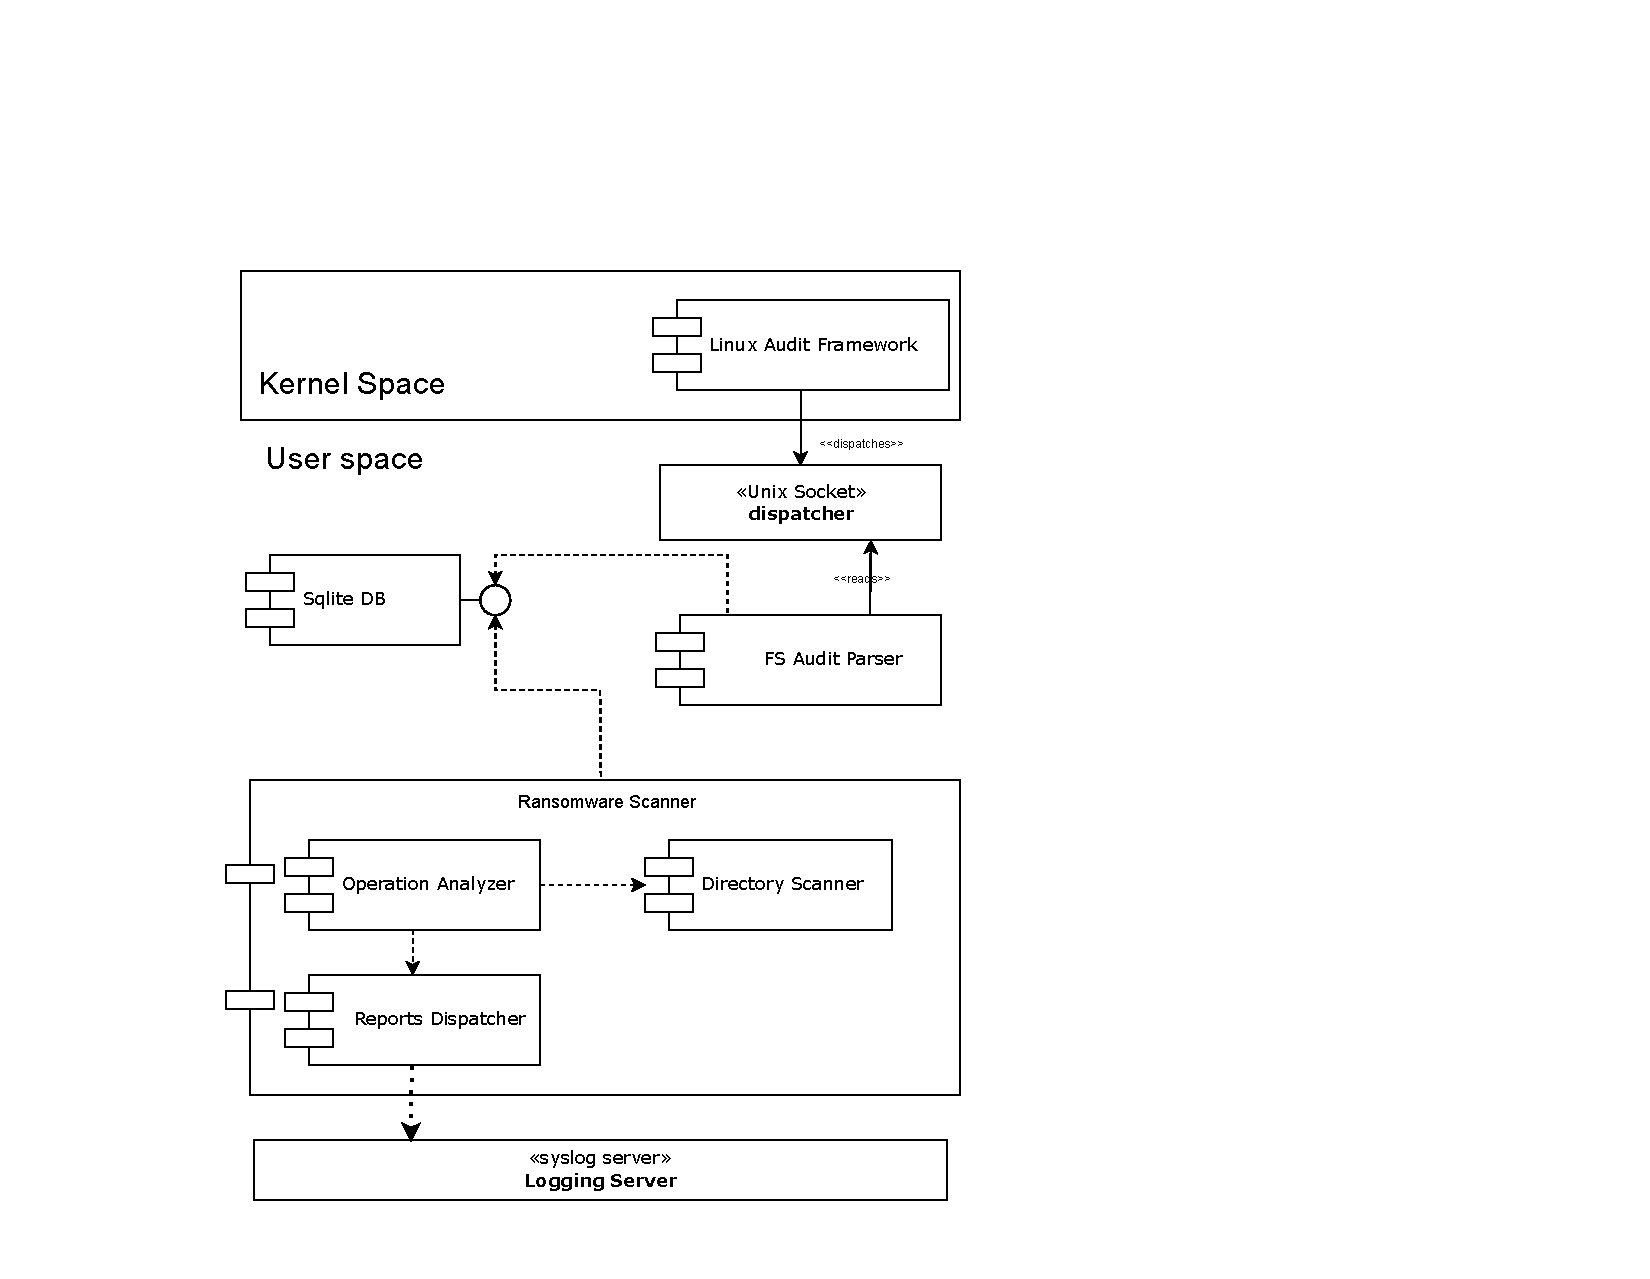
\includegraphics[width=0.52\linewidth]{rysunki/architektura-systemu.drawio.pdf}
    \caption{Diagram obrazujący zależności pomiędzy komponentami~i~źródłami informacji. Komponent \texttt{FS Audit Parser} nie komunikuje się bezpośrednio z komponentem \texttt{Ransomware Scanner}.}
    \label{fig:enter-label}
\end{figure}
Komponent FS Audit Parser odpowiada za zbieranie~i~parsowanie informacji przesyłanych przez \texttt{auditd}, będący częścią Linux Audit Framework, a następnie zapisuje je~w~bazie SQLite.
\newline
Komponent Ransomware Scanner enkapsuluje~w~sobie logikę aktywowania~i~przeprowadzania skanu~w~celu wykrycia ataku. Informacje o systemie są zbierane z bazy danych. Po przeprowadzeniu skanu wysyła on raport do serwera aplikacji \texttt{syslog}.
\newline
FS Audit Parser dokonuje wyłacznie zapisów do bazy, a Ransomware Scanner wyłącznie odczytu. Architektura aplikacji zezwala na dowolną wymianę komponentów nie będących powiązanych bezpośrednio z jej logiką biznesową jak baza danych albo metoda zczytywania wiadomości o systemie plików.

\begin{figure}[H]
    \centering
    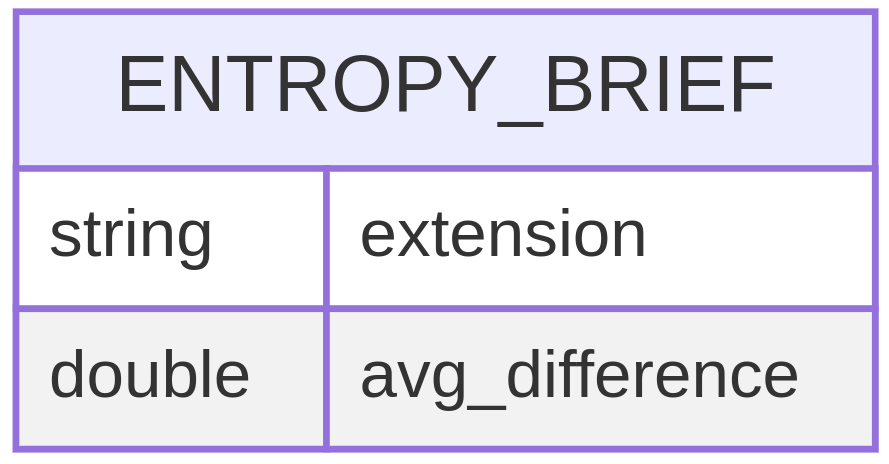
\includegraphics[width=0.3\linewidth]{rysunki/db.png}
    \caption{Schemat bazy danych.}
    \label{fig:enter-label}
\end{figure}
Projekt bazy danych jest bardzo prosty~i~oparty na podstawowych informacjach potrzebnych do implementacji logiki wykrywania ataku zdefiniowanych~w~sekcji \hyperref[sec:wybor]{Wybór odpowiednich statystyk~i~metryk do analizy}. Baza danych ma agregować funkcję przekazywania informacji między komponentami~i~zapisywaniu ich~w~celu prześledzenia danych historycznych na niewielką skalę.
\newline
Projekt architektury ze względu na silnie powiązaną dziedzinę z kontekstem technologicznym, nosi znamię pokrewnej do architektury wdrożenia. Prywatnie uważam,~że~nie jest to problemem gdyż powszechnie stosowane rozwiązania~w~cyberbezpieczeństwie \emph{nie mogą} pozwolić sobie na zupełne wyabstrachowanie swojej architektury od dziedziny technologicznej jaką mają obejmować. 
%%%%%%%%%%%%%%%%%%%%%%%%%%%%%%%%%%%%%%%%%%%%%%%%%%%%%%%%%%%%%%%%%%%
\section{Implementacja algorytmów wykrywających podejrzane działania}
%%%%%%%%%%%%%%%%%%%%%%%%%%%%%%%%%%%%%%%%%%%%%%%%%%%%%%%%%%%%%%%%%%%